\setcounter{chapter}{0}
\textcolor{orange}{\chapter{La Pomme ou le Singe et ses semblables}}
		\begin{wrapfigure}[20]{l}{80px}
	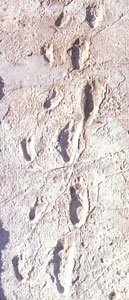
\includegraphics[width=80px]{img7.png}
	\caption{Trace de pas trouvées à Laetoli}
\end{wrapfigure}
\\ \\ \\
	Les traces de pas à Laetoli sont celles d'un homme moderne, c'est la preuve 
	que les hommes n'ont pas évolué et qu'ils ont toujours été présents sur 
	Terre, créés par Dieu.\\ \\
	Petit crédo créationniste qui veut nous faire croire que les hommes et les
	dinosaures ont cohabité !\\ \\  \\

	Plus sérieusement, les traces de pas à Laetoli sont probablement celles d'un 
	australopithèque qui n'est même pas de notre lignée. C'était bien un 
	hominidé bipède qui a marché ce jour-là, mais ce n'est pas un "ancêtre" de 
	l'homme moderne.\\
Les traces de pas de Laetoli ne peuvent pas être celles d'un Homo sapiens, pour 
s'en convaincre il suffit de les comparer visuellement.\\ \\ \\ \\ \\

\section{Les évolutionnistes disent que "l'homme descend du singe"}
\begin{wrapfigure}[13]{r}{110px}
	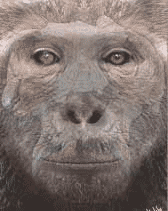
\includegraphics[width=110px]{img8.png}
\end{wrapfigure}
C'est absolument faux, l'homme ne descend pas du singe. C'est un singe lui-même ! 
On attribue, à tort, cette phrase à Charles Darwin et aux scientifiques. 
Ce que l'on sait c'est que les hommes et le chimpanzé ont un ancêtre commun, un 
singe hominoïde. Depuis ce Dernier Ancêtre Commun les espèces se sont séparées
il y a 8 à 9 millions d'années. Les lignées divergentes ont ensuite évolué 
chacune de leur côté. Les gorilles ou les chimpanzés sont donc des cousins 
éloignés de l'homme mais en aucun cas des frères ou des pères!\\ \\
On peut également se poser la question de savoir pourquoi la parenté avec le 
singe est une insulte; Sans doute parce qu'elle rappelle que l'homme est un 
animal parmi d'autres. Ni supérieur, ni inférieur. Cette mise au point gêne 
les extrémistes qui positionnent l'homme au-dessus des autres espèces comme un 
aboutissement. \\
A ce propos il est bon de rappeler que l'histoire de la Terre s'est faite sur 
plusieurs milliards d'années alors qu'Homo sapiens n'apparaît qu'il y a 
seulement 195 000 ans...

\section{La théorie de l'évolution ce n'est qu'une hypothèse}
\begin{wrapfigure}[13]{l}{150px}
	
\includegraphics[width=150px]{img9.png}
\end{wrapfigure}

La biologie avance par hypothèse et théories (comme en chimie, en géologie, en 
génétique). En avançant une hypothèse le scientifique doit vérifier qu'elle 
tient debout, argumenter, trouver des preuves, expérimenter. Un vrai 
scientifique doit accepter que sa théorie soit réfutée, contredite, 
ce n'est pas pour cela qu'elle est fausse ! \\
Sans théorie ni hypothèse nous penserions toujours que la Terre est plate!\\
La théorie de l'évolution est aujourd'hui vérifiée par les faits, les fossiles, 
les expériences. Cela n'empêche pas que des scientifiques puissent continuer 
à travailler le sujet, comme n'importe quelle théorie. \\
Le créationniste, quelle que soit sa religion, ne se base pas sur des faits mais
généralement sur un livre qui présente non pas une théorie mais une histoire. 
Le fait d'être croyant n'empêche d'ailleurs pas de prendre la théorie de 
l'évolution en considération. \textit{Le Pape Jean Paul II a lui même reconnu 
	que la théorie de l'évolution n'était pas qu'une hypothèse}.\\

Depuis 1987, une nouvelle forme de créationnisme voit le jour aux États-Unis, le 
Dessin Intelligent (ou Intelligent Design). Le but avoué est de faire enseigner
le Dessin Intelligent dans les écoles américaines en se parant d'une apparence 
scientifique. Ces partisans remplacent la notion de Dieu par celle de l'être 
supérieur pour expliquer que l'harmonie de notre monde ne peut s'expliquer que 
par une intervention extérieure, c'est-à-dire divine !	
	\begin{figure}[h]
		\begin{center}
	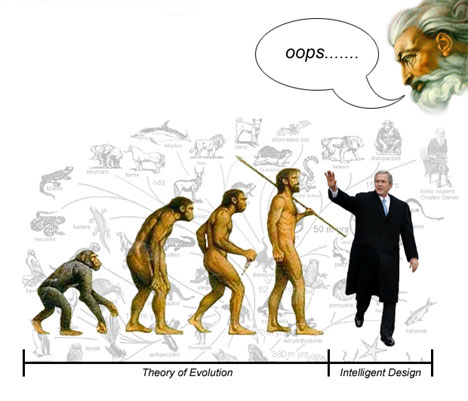
\includegraphics[width=250px]{img10.png}
	\caption{Théorie de l'évolution}
		\end{center}
	\end{figure}	
	
\textcolor{orange}{\chapter{Une lecture nouvelle de théories religieuses}}
Depuis quelques temps, les hommes d'église nous propose une nouvelle façon 
d'aborder les écrits religieux, Pie XII (pape de 1939 à 1958), Jean Paul II 
(pape de 1978 à 2005) longuement critiqué à ce sujet notamment par les 
Créationnistes, ils ont été les prédécesseurs de ce mouvement de lecture nouvelle.
Plusieurs ouvrages également ont été édité comme "Une Nouvelle Lecture Biblique"
de Simon Hazan et Antoine Mercier (édité chez Lichma en 2010), 
"Divine Chamaillerie" de Sébastien Allali (édité chez Lichma en 2010).\\
Mais tout cela est une question d'interprétation, nous allons pour rester dans 
notre sujet  prendre et expliquer certains passages et certaines images qui se 
lie le plus avec la Science.\\
Tout d'abord, la création du monde, précédemment nous l'estimions à quinze milliards
d'années et la Bible en sept jours or partons du principe qu'un jour ne soit pas un
jour réel mais un jour Divin prenons le $6^{éme}$ jours création des animaux 
domestiques, des reptiles et des serpents, du premier homme et la femme toutes
ces choses là sont dans un stade final au niveau de l'évolution  et si chaque 
jour divin représentait un à deux milliards d'années plutôt surprenant car cela 
colle exactement aux estimations des scientifiques à cette étape 
d'évolution et rajoutons maintenant les six autres jours divins, nous arrivons à
un total de sept à quatorze milliards d'années ! 
Cela ne vous rappelle rien? Une fois de plus une hypothèse qui se
laisse imaginer.\\ \\

\begin{wrapfigure}[9]{r}{110px}
	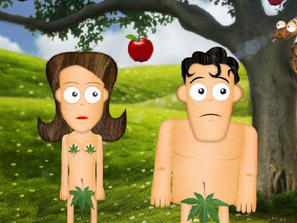
\includegraphics[width=110px]{img11.png}
\end{wrapfigure}
Si nous continuons avec Adam et Ève (s'ils ont existé) leurs ages étaient estimé 
à 930 ans ce qui peut paraitre aberrant et impossible, cependant si nous partons 
du principe une nouvelle fois que cette age fut compté en mois cela ne ferait 
plus que soixante-dix sept ans. \\
Un peu plus crédible ?\\
Terminons avec le Jardin d Éden et l'arbre Sacré, lieu où vivaient Adam et Ève
immortel à la condition qu'ils étaient défendu de croquer la moindre pomme sous 
peine d'être exclu d Éden (tout comme Satan).\\
L'image que nous pouvons faire du Jardin d Éden et de l'immortalité qu'elle 
regorgeait ne serait pas lié directement à Adam et Ève mais à l'Humanité 
autrement dit la fécondité, s'ils se reproduisent et que chaque générations 
fait de même nous trouvons ici une sorte d'immortalité de la race humaine.\\
L'arbre quant à lui referme la nature de l'Homme, le fait de prendre une pomme 
montre qu'il veut toujours plus que ce qu'il n'a, le confort, toujours plus 
de savoir, toujours plus d'évolution et de technologie, le matérialisme, la 
conquête et la recherche de la supériorité ... \\Tout cela sans se soucier du mal
qui l'engendre et de la détérioration d'autrui et de son monde.


